% Multiple time periods -- the first of four composite figures for Lecture 7
% (collocation).  Prof. Dowling, 2026-09-08: "one composite figure per main
% idea ... We can show these illustrations using tikz."
%
% WHAT IT SHOWS.  collocation.tex writes the dynamic optimization problem over
% a single period and then notes "Biegler writes Eq. 7-1 over $N_T$ time
% periods; we use the single-period form."  That sentence is the only place the
% multi-period structure appears, so this figure carries it: the horizon
% [t_0, t_f] is cut at T_1, ..., T_{N_T-1}, each period k gets its OWN control
% profile u^{(k)}(t), and the differential states are what tie the periods
% together -- z is continuous across every junction while u is free to jump.
% That asymmetry (states continuous, controls not) is the whole point, and it
% is why the picture has two lanes rather than one.
%
% Biegler, Nonlinear Programming (2010), Ch. 8, Eq. (8.5) and the surrounding
% discussion of the multi-period form.
%
% GREYSCALE.  Two curves, two hues (Okabe-Ito blue L*=46, orange L*=70.6, so
% dL* = 24.6 -- separated in print on hue alone), AND two line styles (z solid,
% u dashed), AND both are directly labelled at the curve.  Three redundant
% encodings; nothing is carried by colour alone.  See figures/README.md.
%
% TIKZ LIBRARIES.  Base tikz only.  No \calc, no patterns, no
% decorations.pathreplacing -- the course pack's preamble.tex and this
% directory's preamble.tex load DIFFERENT library sets, and this figure stays
% inside the intersection so it builds both ways.

\definecolor{cpblue}{HTML}{0072B2}
\definecolor{cporange}{HTML}{E69F00}

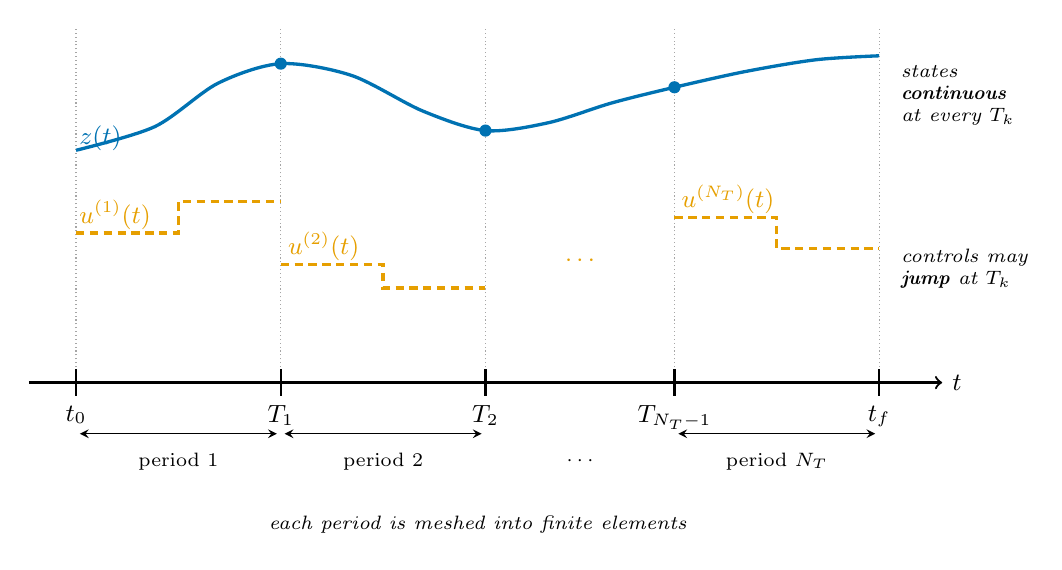
\begin{tikzpicture}[x=1cm, y=1cm, font=\small]

  % ---------------------------------------------------------------- geometry
  % Period boundaries.  The gap between 5.8 and 8.2 is the "..." region.
  % t0 = 0.6, T1 = 3.2, T2 = 5.8, T_{NT-1} = 8.2, tf = 10.8.

  % Vertical rules at the junctions, spanning both lanes.  Drawn FIRST so the
  % curves sit on top of them.
  \foreach \x in {0.6, 3.2, 5.8, 8.2, 10.8}
    \draw[black!35, densely dotted] (\x,-0.35) -- (\x,4.15);

  % ------------------------------------------------------- lane 1: the states
  \draw[cpblue, very thick]
    plot[smooth] coordinates {(0.6,2.6) (1.6,2.9) (2.4,3.45) (3.2,3.7)
      (4.1,3.55) (5.0,3.1) (5.8,2.85) (6.6,2.95) (7.4,3.2) (8.2,3.4)
      (9.1,3.6) (10.0,3.75) (10.8,3.8)};
  \foreach \x/\y in {3.2/3.7, 5.8/2.85, 8.2/3.4}
    \fill[cpblue] (\x,\y) circle (2.2pt);
  \node[cpblue, above right, inner sep=1pt] at (0.6,2.55) {$z(t)$};
  \node[right, align=left, font=\scriptsize\itshape, inner sep=2pt]
    at (11.0,3.3) {states\\ \textbf{continuous}\\ at every $T_k$};

  % ----------------------------------------------------- lane 2: the controls
  % Piecewise-constant sketch: each period carries its own profile, and the
  % profile is allowed to JUMP at a junction.  Dashed, so the distinction from
  % z(t) survives a photocopy.
  \draw[cporange, very thick, densely dashed]
      (0.6,1.55) -- (1.9,1.55) -- (1.9,1.95) -- (3.2,1.95);
  \draw[cporange, very thick, densely dashed]
      (3.2,1.15) -- (4.5,1.15) -- (4.5,0.85) -- (5.8,0.85);
  \draw[cporange, very thick, densely dashed]
      (8.2,1.75) -- (9.5,1.75) -- (9.5,1.35) -- (10.8,1.35);
  \node[cporange, above right, inner sep=1pt] at (0.6,1.55) {$u^{(1)}(t)$};
  \node[cporange, above right, inner sep=1pt] at (3.25,1.15) {$u^{(2)}(t)$};
  \node[cporange, above right, inner sep=1pt] at (8.25,1.75) {$u^{(N_T)}(t)$};
  \node[right, align=left, font=\scriptsize\itshape, inner sep=2pt]
    at (11.0,1.1) {controls may\\ \textbf{jump} at $T_k$};

  % The unmodelled middle periods.  The dots go in the CONTROL lane only: z(t)
  % is drawn unbroken all the way across, which is the figure's whole claim.
  \node[cporange] at (7.0,1.2) {$\cdots$};

  % --------------------------------------------------------------- time axis
  \draw[->, thick] (0,-0.35) -- (11.6,-0.35) node[right] {$t$};
  \foreach \x in {0.6, 3.2, 5.8, 8.2, 10.8}
    \draw[thick] (\x,-0.52) -- (\x,-0.18);
  \node[below] at (0.6,-0.52)  {$t_0$};
  \node[below] at (3.2,-0.52)  {$T_1$};
  \node[below] at (5.8,-0.52)  {$T_2$};
  \node[below] at (8.2,-0.52)  {$T_{N_T-1}$};
  \node[below] at (10.8,-0.52) {$t_f$};

  % ------------------------------------------------------- period labels
  \node[font=\scriptsize] at (1.9,-1.35)  {period $1$};
  \node[font=\scriptsize] at (4.5,-1.35)  {period $2$};
  \node[font=\scriptsize] at (7.0,-1.35)  {$\cdots$};
  \node[font=\scriptsize] at (9.5,-1.35)  {period $N_T$};
  \foreach \a/\b in {0.65/3.15, 3.25/5.75, 8.25/10.75}
    \draw[<->, >=stealth] (\a,-1.0) -- (\b,-1.0);

  % Each period is itself meshed into finite elements -- the next figure.
  \node[align=center, font=\scriptsize\itshape] at (5.7,-2.15)
    {each period is meshed into finite elements};

\end{tikzpicture}
